\chapter {Data} \label{chap:data}


This chapter will introduce the data provided by the DI, and the processing steps necessary to anonymize and prepare the data for use in classification rule learning.
Section \ref{chap:data:cleaning} details the anonymization and bias-removal steps.
Next, Section \ref{chap:data:layout} introduces a naming convention and describes the format of the data before and after the initial aggregation. Section \ref{chap:data:labelling} will detail the chronic label.

\section{Data Anonymization and Cleaning} \label{chap:data:cleaning}

This work was carried out using data collected at the DI between July 1, 2007, and January 20, 2020. The data set contains 34,577 unique clients with a total of 5,393,987 recorded interactions with the DI. The data is organized into one table that covers all clients. Each row of the table contains a single interaction with the shelter, which can be a sleep event, a meeting with a counsellor (addiction services, career services, etc.), a log of some interaction, or an event resulting in a variable-length ban. Interactions have a timestamp, a unique client ID and a unique table index.
The data anonymization and a client privacy protocols used in this work were approved by the University of Calgary Conjoint Faculties Research Ethics Board. 
Following the procedure put forth by Kuhn and Culhane \cite{kuhn1998applying}, the data was pruned to mitigate the effects of left-truncation and right-censor bias.

Censoring is the effect that comes from the discrete start and end of data collection.  That is, a client who accesses shelter services before July 1, 2007, will have the initial portion of their access records missing. Any client who is not identified as chronic prior to January 20, 2018, will be potentially mislabeled because they could become chronic after January 20, 2018. These effects are called left-truncation bias and right-censor bias respectively.

Left-truncation bias results from the sharp cut-off at the start of data collection.
In the context of this work, there will be individuals who are chronic at the start of the data collection but any analysis will not see this and determine that the individual is a new client. The DI started collecting sleep records on July 1, 2008, thus we set the left-truncation bias cut-off to July 1, 2009, and remove any client that slept at the DI before that date. The assumption is that clients within one year of the start of data collection have a higher probability of having accessed DI services prior to the beginning of data collection.

Right-censor bias is a result of filtering clients who continue to access the shelter after the end of the data record. These clients might become chronic after the end of the available data, meaning any system is likely to classify them incorrectly. Thus we set the right-censor bias cut-off to January 20, 2018.

When performing the right-censor bias adjustment there are two appropriate methods. The first being to remove all clients that have a recorded interaction after the cut-off date. The other is to remove only the clients who have their first interaction (in this work, sleep interactions were used) after the cut-off date. The first method minimizes the number of individuals who become chronic that are mislabelled as not chronic at the cost of having fewer individuals in the data set. The second method retains more individuals in the data set but has a higher risk of mislabelling a few individuals. In this work, the second method was used as it resulted in a larger number of identified chronic individuals.

% Fortunately, these methods can be compared using historical data. As with the main work, this analysis will be performed using data after the censor bias mitigation efforts, with cut-off dates of July 1, 2009 and January 20, 2018 for the left-truncation and right-censor respectively. 

% To properly compare these two methods, it is necessary to make an estimate of the false non-chronic count using the first method and the additional true-chronic individuals identified using the second method. The latter value is much easier to calculate as it is simply the difference between the number of classified individuals when using each method. Performing this simple analysis tells us that there is a difference of 593 clients identified as chronic (884 vs 291).

% Estimating the false non-chronic count is more difficult. Individuals that are falsely classified as non-chronic because of the right censor bias, are those who eventually become chronic after the data collection date (January 20, 2020), with the cut-off date set to 2018. Which gives clients two years to become chronic in the worst case (the worst case is a client who first accesses shelter services in January 19, 2018). Using this we can generate an approximate upper bound on the number of missed clients.

% The upper bound can be estimated by observing the probability that an individual is identified as chronic after two or more years, and making the assumption that all clients from some period prior to January 20, 2018 all enter for the first time on January 19, 2020. For this work we will look at the period from January 20, 2016 - January 19, 2018. This includes a total of 5208 clients. Over the entire data set it was observed that \~1.84\% of clients become chronic after two or more years. Which gives the upper bound of $5208 \cdot 0.184 = 96 \text{ individuals}$ . A lower bound can be similarly computer by assuming all 5208 clients entered on January 20, 2016. ~0.818\% of clients become first chronic after four years, applying this gives  $5208 \cdot 0.0818 = 43 \text{ individuals}$ . 

% Finally, comparing the two methods it is observed that the first method results in 593 fewer identified chronic clients (a reduction of 67\%) but results in upwards of 100 fewer mis-classified individuals. In this work, the second method will be used, as having more than three times as many chronic individuals identified will help the learning algorithm.

Thus, any client that starts sleeping at the DI after January 20, 2018, is removed from the data set.
This reduced the clients covered down to 18,398, representing a 46.8\% reduction in the number of clients.



\section{Data Layout and Transformations} \label{chap:data:layout}

% Original (RAW) data table $T$
% Client data table (These are called attributes) $A$ (num_df)
% Individual attributes are labelled $a_1, a_2, ..., a_L$
% Coverage Table (features) $\mathcal{F}$
% Each column represents a feature (/single rule) $f_i$
% class labels (true/false) $c$
% predicted labels $\hat c$

\subsection{DI Data Table}


The data collected at the DI comes as one data table $T$, where columns contain data points being tracked (e.g. ClientID) and each row contains one interaction with the DI for a total of 2,184,854 interactions. Table \ref{tbl:university} outlines each column and the type of data that it can contain. The EntryType column details why each event was logged. For example, an EntryType of Bar is recording that the client was banned from the DI on that specific day. The Bar duration is not used in this work. Similarly CounsellorsNotes, ProgressDetails, and Log correspond to three different instances of entering a written log into the database. For privacy reasons the log text is not used. Sleep events occur when a client accesses the DI to sleep.


\begin{table}[h!]
	\begin{tabular}{ c c p{0.7\textwidth} } 
		\toprule
		Column name & Values &  \\
		\midrule
		ClientId & \emph{integer} & Unique to each client \\
		Date & \emph{date} & Date of interaction \\
		Age & \emph{integer} & Client's age at the time of data export \\
		EntryType & \emph{string} & One of 'Bar', 'CounsellorsNotes', 'ProgressDetails', 'Log', 'Sleep' \\
		EmployeeIsCounsellor & \emph{boolean} & Is the employee logging the interaction a counsellor? \\
		EmsLogFlag & \emph{boolean} & Were EMS called for this client? \\
		PoliceLogFlag & \emph{boolean} & Were the police called on account of this client? \\
		\bottomrule
	\end{tabular}
	\caption{Description of data ($T$) provided by the DI.}
	\label{tbl:university}
\end{table}


Missing or invalid data can introduce a large amount of error in the final classifications, and it is thus necessary to discuss what is done when presented with missing or invalid data. The data used in this work has been exported from the DI after having undergone some preliminary cleaning. The cleaning was performed before being exported at the DI, the raw data was not observed in this work. This means the data $T$ can be trusted to only contain valid values (e.g. all counts are positive, there are no null values, etc.). 

Another source of potential bias is the existence of the diversion services team at the DI. This team is responsible for identifying chronic individuals and individuals at risk for chronic homelessness and helps transition them into housing following housing first principles. This is considered to be a small source of bias in this work as the diversion services team is relatively new. Housing first in Canada was heavily influenced by the At Home/Chez Sois study which concluded in 2014 \cite{athome2014chezsoi}.

\subsection{Data Transformations}

The data format described above is not sufficient for use with our classification rule learning system and is not yet suitable to perform all but the most basic analysis. A better format would be a table where each client is a row and each column is an attribute describing the client.
This new table is called $A$ and has a length of 18,398 (the total number of clients).
Each attribute of $A$ is denoted $a$, where $a_i$ denotes the $i$th column name of $A$. The minimum and maximum values of attribute $a$ are denoted $min(a)$ and $max(a)$ respectively. Each attribute $a$ is a summary of interactions that a client has recorded in $T$. For example, a common attribute is 'Sleep' which records the total number of times a client has an EntryType of Sleep in $T$.
The table $A$ has nine columns (attributes), Age, Bars, CounsellorsNotes, EmployeeIsCounsellor, EmsLogFlag, Log, PoliceLogFlag, ProgressDetails, Sleep.



The nine columns of $A$ are derived from the seven columns in $T$. Not all the columns in $T$ are directly used as attributes. Some columns are combined to create an attribute. For example, the Date column does not become an attribute but is used together with the Age column to calculate a client's age at the first interaction with the DI.
The Age column in $T$ represents client age when the data was exported (2020). To get the actual age at the time of interaction, the Date field is used to calculate the client's approximate age. As a matter of anonymity, the client's birth dates are unknown, which means the Age attribute is only accurate to one year.
The EntryType column is a categorical column with five options 'Bar', 'CounsellorsNotes', 'ProgressDetails', 'Log', and 'Sleep'. This column is split into five attributes with each attribute counting the number of times a client had an EntryType equal to that attribute.
The EmployeeIsCounsellor, EmsLogFlag, and PoliceLogFlag columns each become separate attributes that count the number of times these flags were set in $T$.


As the purpose of this work is to classify individuals as soon as possible, the entire attribute table will not be used when making classifications. Instead, a modified attribute table will be used that is generated using only a client's first $d$ days after first sleeping at the DI. 
This is fortunately a simple procedure. Instead of making the transformation of $T \rightarrow A$ an additional procedure that filters out client interactions $d$ days after the client's first sleep is introduced. The new transformation is $T \rightarrow A_d$ where $A_d$ represents the attribute table for each client's first $d$ days after sleeping at the DI. For example, the attribute table that represents a client's first 14 since sleeping at the DI is denoted $A_{14}$.

 The $A_d$ table has an additional seven columns, which represent the count of the non-sleep and non-age attributes prior to a clients first sleep at the DI. This means the $A_d$ table has 16 columns Age, Bars, CounsellorsNotes, EmployeeIsCounsellor, EmsLogFlag, Log, PoliceLogFlag, ProgressDetails, Sleep, Bars\_before, CounsellorsNotes\_before, EmployeeIsCounsellor\_before, EmsLogFlag\_before, Log\_before, PoliceLogFlag\_before, and ProgressDetails\_before.


\subsection{Exploratory Data Analysis} \label{chap:data:characteristics}

The attribute table $A_d$ introduced in the previous section is in a form that makes a basic exploratory data analysis possible. For this exploratory data analysis, a $d$ of 30,000 days is used. 30,000 days is larger than the entire data set, so the attribute table $A_{30,000}$ will include all data about a client from their first sleep, until the last day of available data.

Table \ref{tbl:stats:notchronic} includes a summary of the nine attributes along with five additional fields, here called demographics. These fields are Interactions, Tenure, Usage, Average Gap Length, and Episodes. Interactions are a simple count of each recorded interaction a client has with the DI (all EntryTypes). Tenure is the total number of days between a client's first and last interaction with the DI. Usage is the percentage of days that a client accesses DI services, a high usage is indicative of a heavy shelter user, or an individual with a short homeless stint. Average Gap Length is the average gap between stays at the DI, a low Average Gap Length can indicate a heavy user of DI services. Episodes track a client's total number of homeless episodes, where an episode is a grouping of shelter sleeps with a gap between sleeps not exceeding 30 days.

It can be seen from Table \ref{tbl:stats:notchronic} that, while there is a large range of values from each attribute (and demographic), most client experiences are grouped toward the lower end. Figures \ref{fig:pdf} and \ref{fig:demopdf} demonstrate the distribution of these values. This reinforces that the majority of clients that access shelter services only do so a small number of times, in fact, Figure \ref{fig:pdf} shows that the vast majority of clients spend less than 10 nights sleeping at the DI.


\begin{table}[h]
	\centering

	\begin{tabular}{lrrrr}
	\toprule
	Attributes													 &        min &   max &     mean &   median \\
	\midrule
	Age                          &          0 &   119 &    38.79 &       37 \\
	Bar (Count)                  &          0 &    68 &     1.05 &        0 \\
	CounsellorsNotes (Count)     &          0 &   443 &     3.72 &        0 \\
	EmployeeIsCounsellor (Count) &          0 &   464 &     6.25 &        0 \\
	EmsLogFlag (Count)           &          0 &    27 &     0.12 &        0 \\
	Log (Count)                  &          0 &  2419 &     7.23 &        0 \\
	PoliceLogFlag (Count)        &          0 &    23 &     0.13 &        0 \\
	ProgressDetails (Count)      &          0 &   539 &     4.77 &        0 \\
	Sleep (Count)                &          1 &  3575 &    82.95 &        5 \\
	\midrule
	Demographics								 &         &    &      &    \\
	\midrule
	Interactions (Count)         &          1 &  5247 &   118.75 &      8.0 \\
	Tenure (Days)                &          1 &  3800 &  650.526 &      138 \\
	Usage (\%)                    &  0.0541859 &   100 &  48.5072 &  34.0721 \\
	Average Gap Length (Days)    &          1 &  3690 &  135.634 &    11.25 \\
	% Stays (Count)                &          1 &  3575 &   82.949 &        5 \\
	Episodes (Count)             &          1 &    31 &  2.74611 &        2 \\
	\bottomrule
	\end{tabular}

	\caption{Basic Attribute statistics and Demographic data for the entire population.}
	\label{tbl:stats:notchronic}
\end{table}

\begin{figure}[ht]
  \figuretitle{Attribute Histograms}
  \centering

	\begin{subfigure}[b]{0.3\textwidth}
    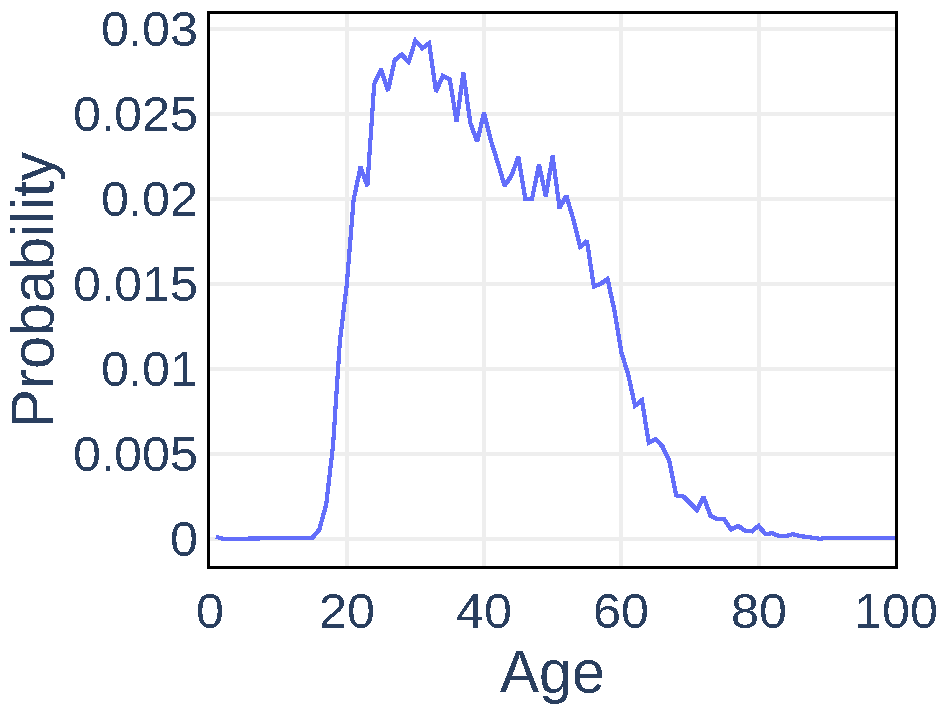
\includegraphics[width=\textwidth]{Figures/Data-Age-PDF}
  \end{subfigure}
	\begin{subfigure}[b]{0.3\textwidth}
    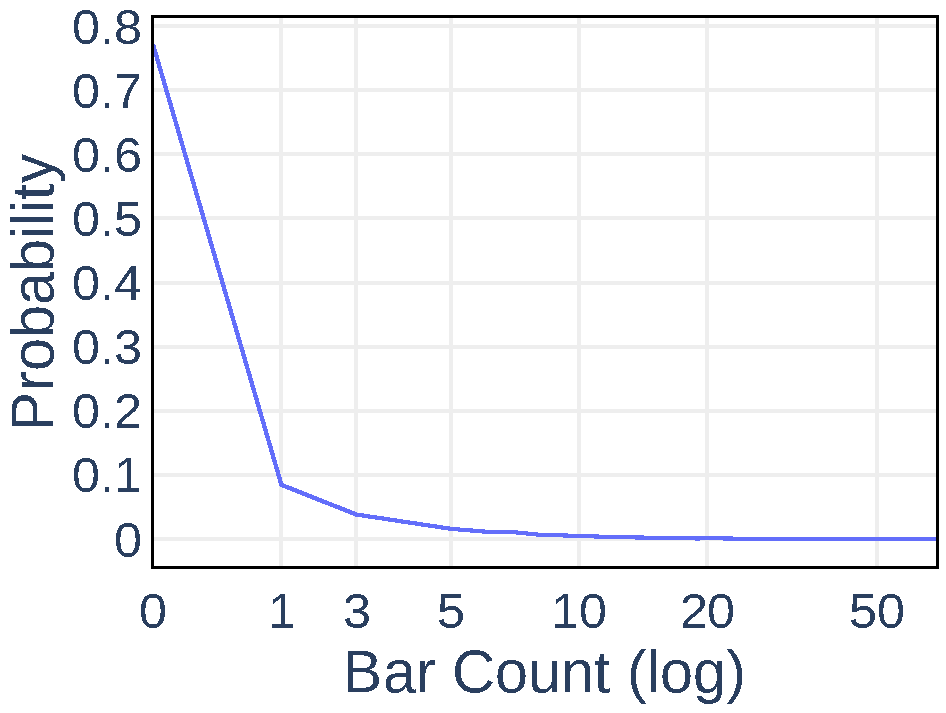
\includegraphics[width=\textwidth]{Figures/Data-Bar-PDF}
  \end{subfigure}
	\begin{subfigure}[b]{0.3\textwidth}
    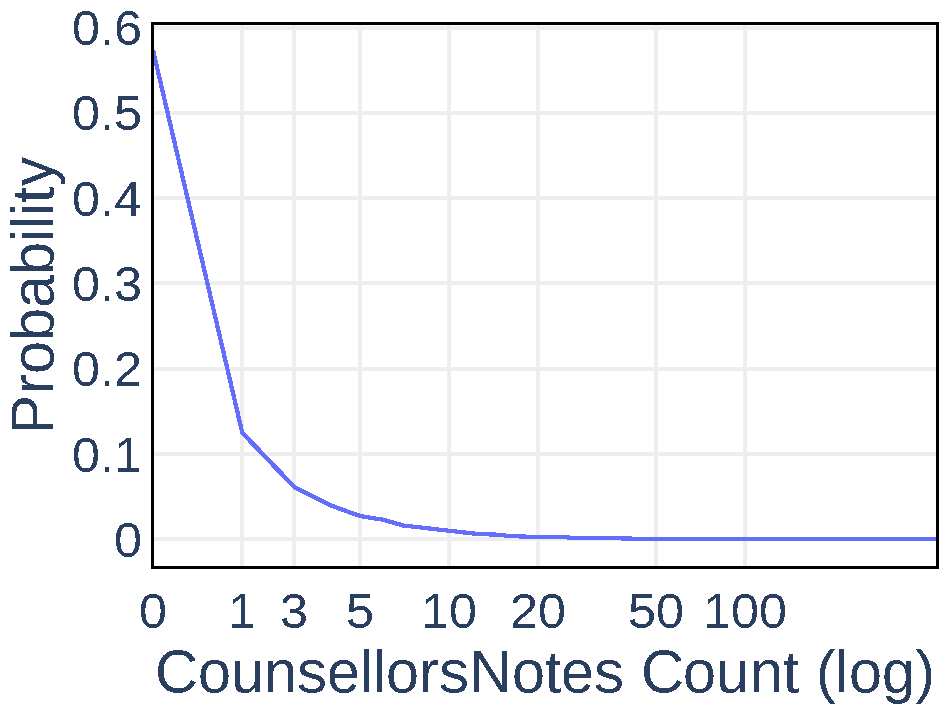
\includegraphics[width=\textwidth]{Figures/Data-CounsellorsNotes-PDF}
  \end{subfigure}
	\vspace*{1em}

	\begin{subfigure}[b]{0.3\textwidth}
    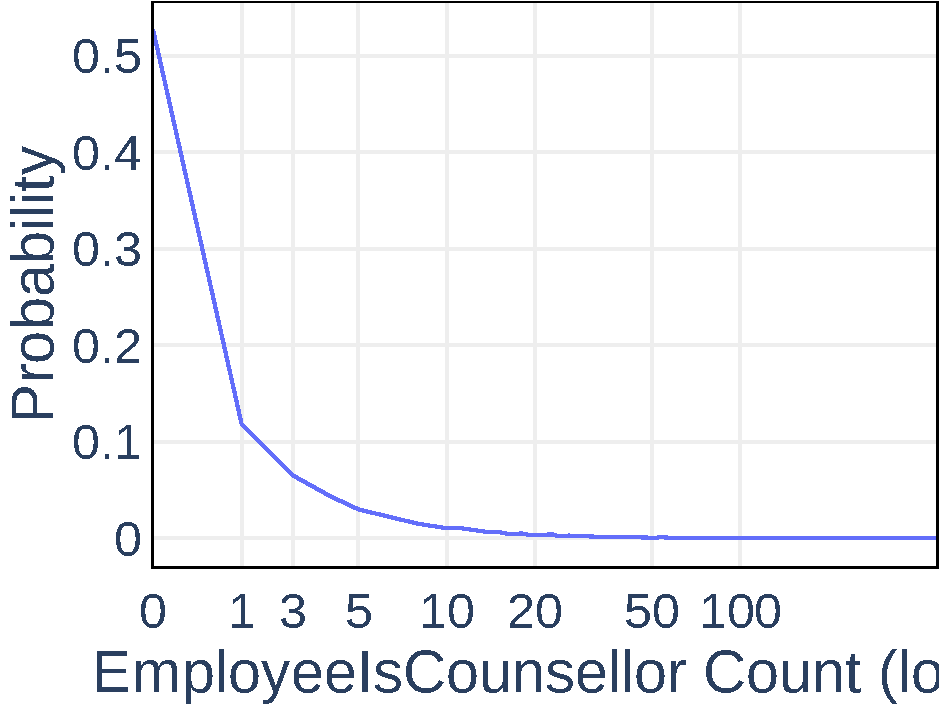
\includegraphics[width=\textwidth]{Figures/Data-EmployeeIsCounsellor-PDF}
  \end{subfigure}
	\begin{subfigure}[b]{0.3\textwidth}
    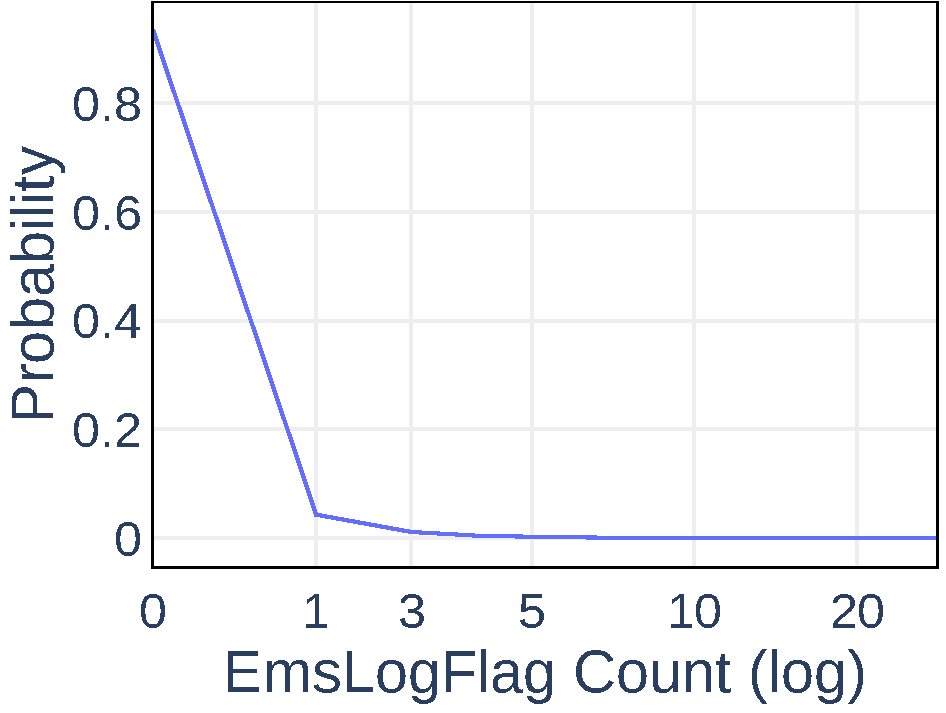
\includegraphics[width=\textwidth]{Figures/Data-EmsLogFlag-PDF}
  \end{subfigure}
	\begin{subfigure}[b]{0.3\textwidth}
    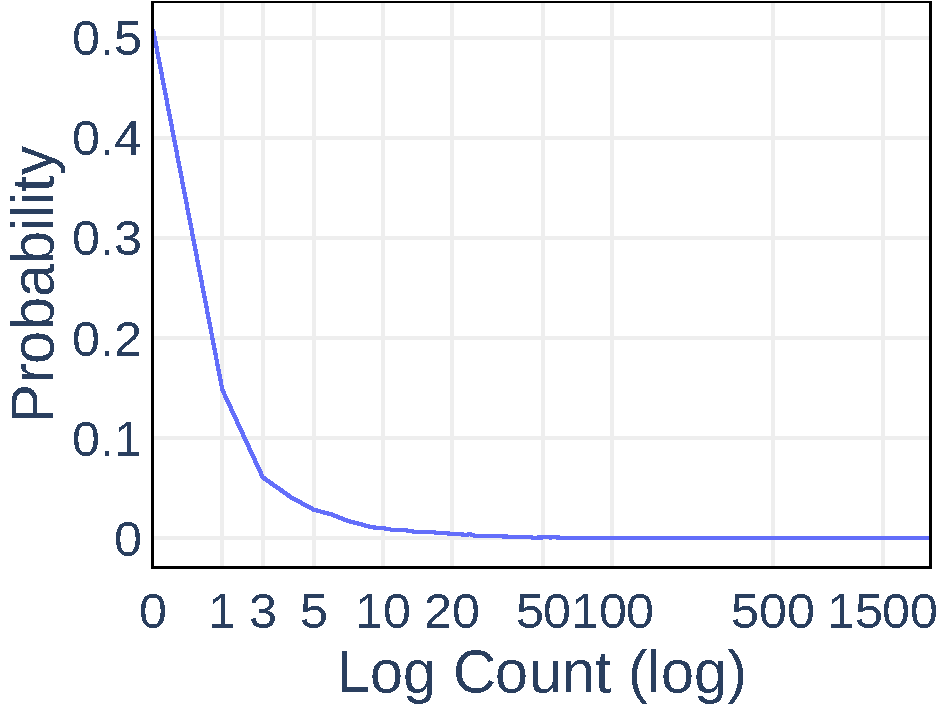
\includegraphics[width=\textwidth]{Figures/Data-Log-PDF}
  \end{subfigure}
	\vspace*{1em}

	\begin{subfigure}[b]{0.3\textwidth}
    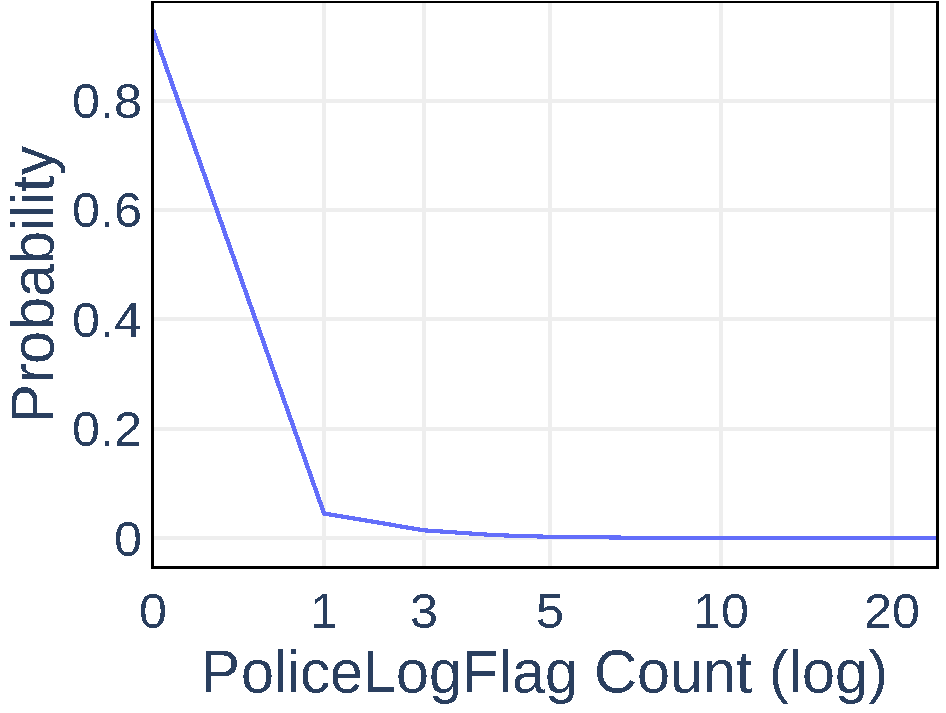
\includegraphics[width=\textwidth]{Figures/Data-PoliceLogFlag-PDF}
  \end{subfigure}
	\begin{subfigure}[b]{0.3\textwidth}
    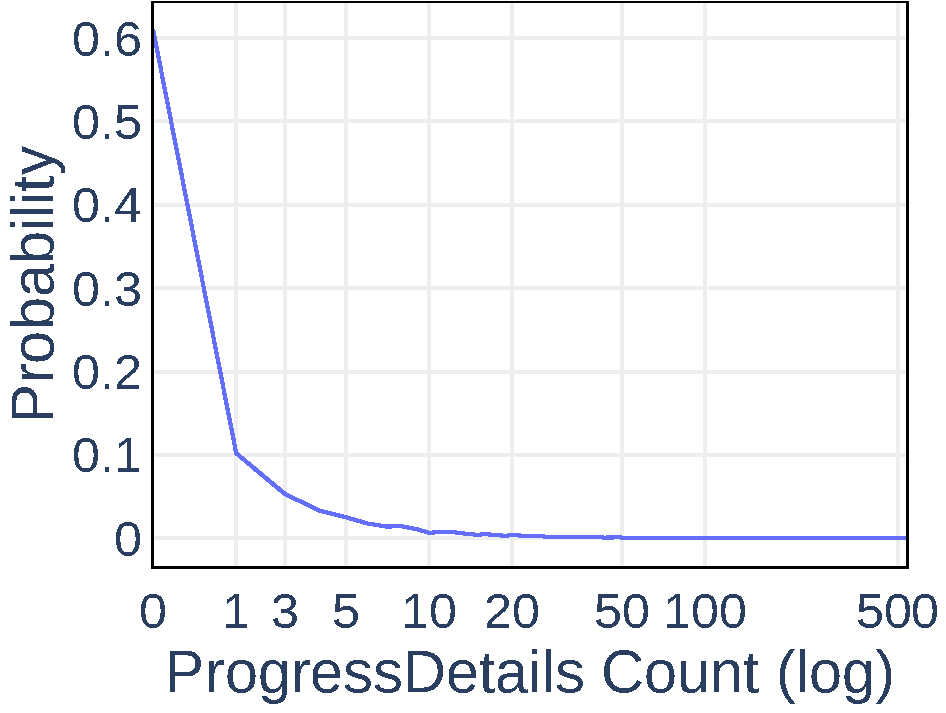
\includegraphics[width=\textwidth]{Figures/Data-ProgressDetails-PDF}
  \end{subfigure}
	\begin{subfigure}[b]{0.3\textwidth}
    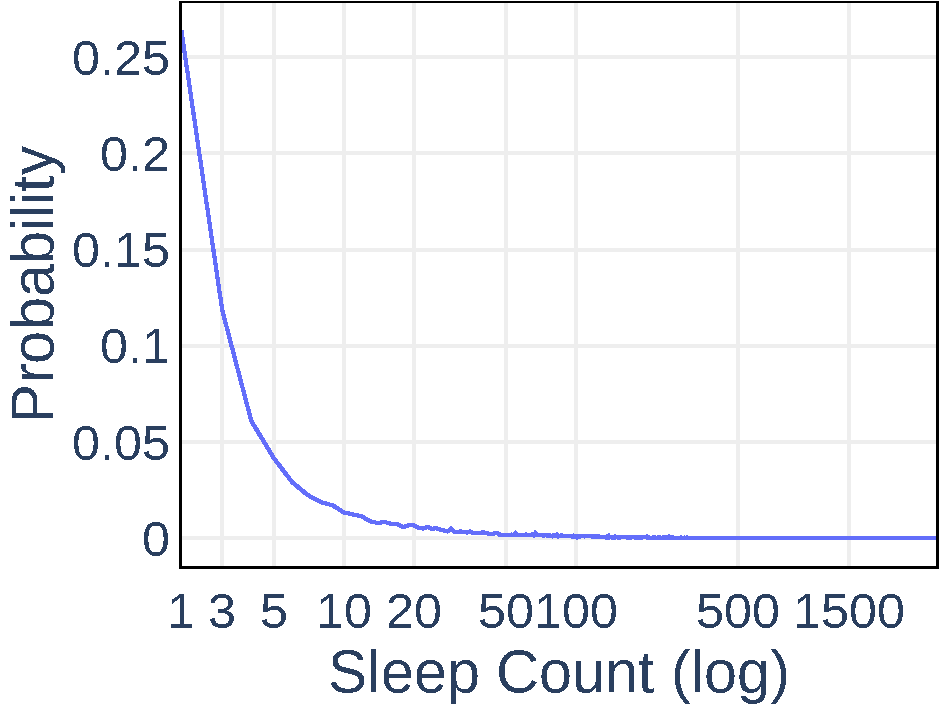
\includegraphics[width=\textwidth]{Figures/Data-Sleep-PDF}
  \end{subfigure}
	\caption{Histograms of the nine attributes.}
	\label{fig:pdf}
\end{figure}

\begin{figure}[ht]
  \figuretitle{Demographic Histograms}
  \centering

	\begin{subfigure}[b]{0.3\textwidth}
    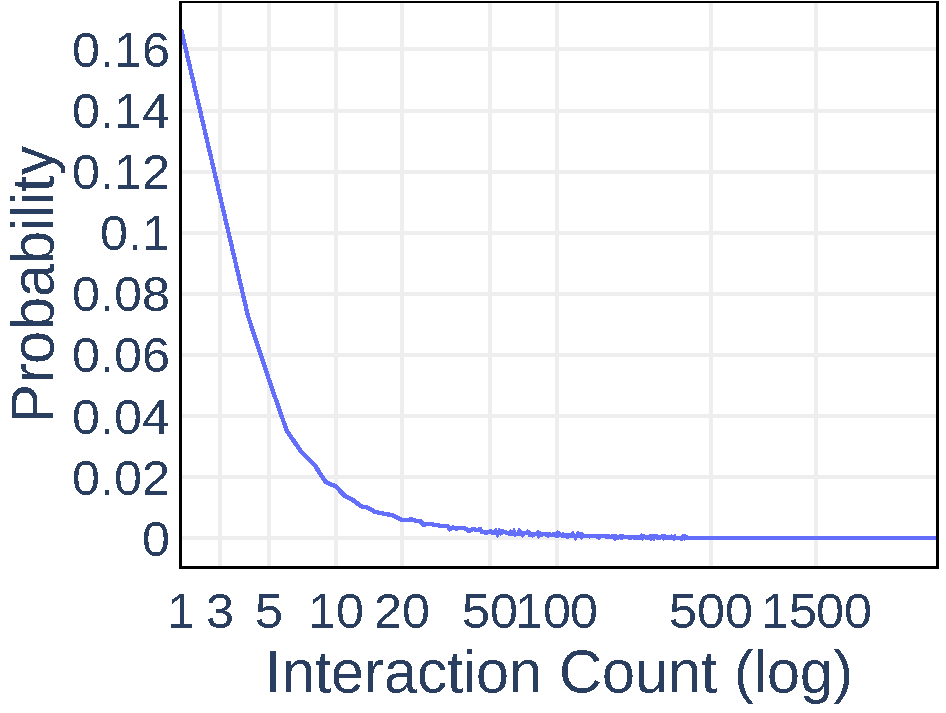
\includegraphics[width=\textwidth]{Figures/Data-Interaction-PDF}
  \end{subfigure}
	\begin{subfigure}[b]{0.3\textwidth}
    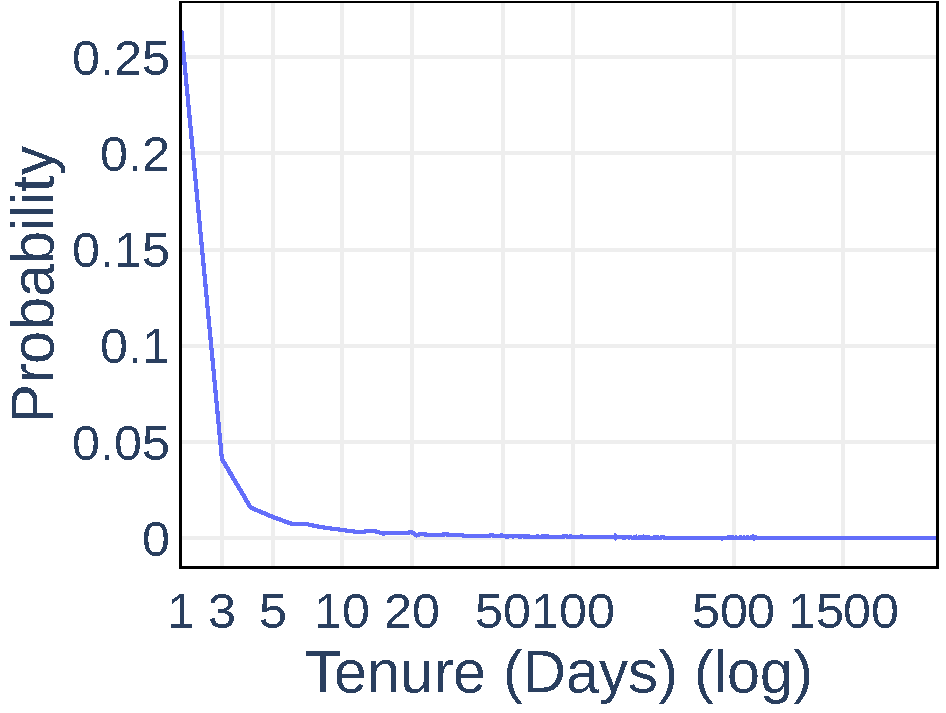
\includegraphics[width=\textwidth]{Figures/Data-Tenure-PDF}
  \end{subfigure}
	\begin{subfigure}[b]{0.3\textwidth}
    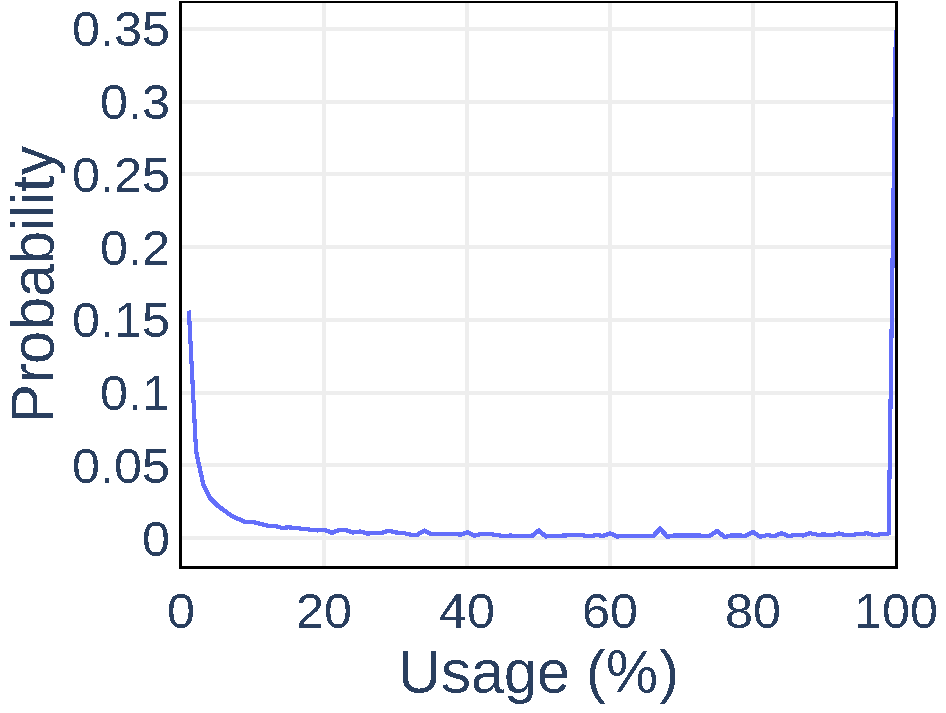
\includegraphics[width=\textwidth]{Figures/Data-UsagePct-PDF}
  \end{subfigure}
	\vspace*{1em}

	\begin{subfigure}[b]{0.3\textwidth}
    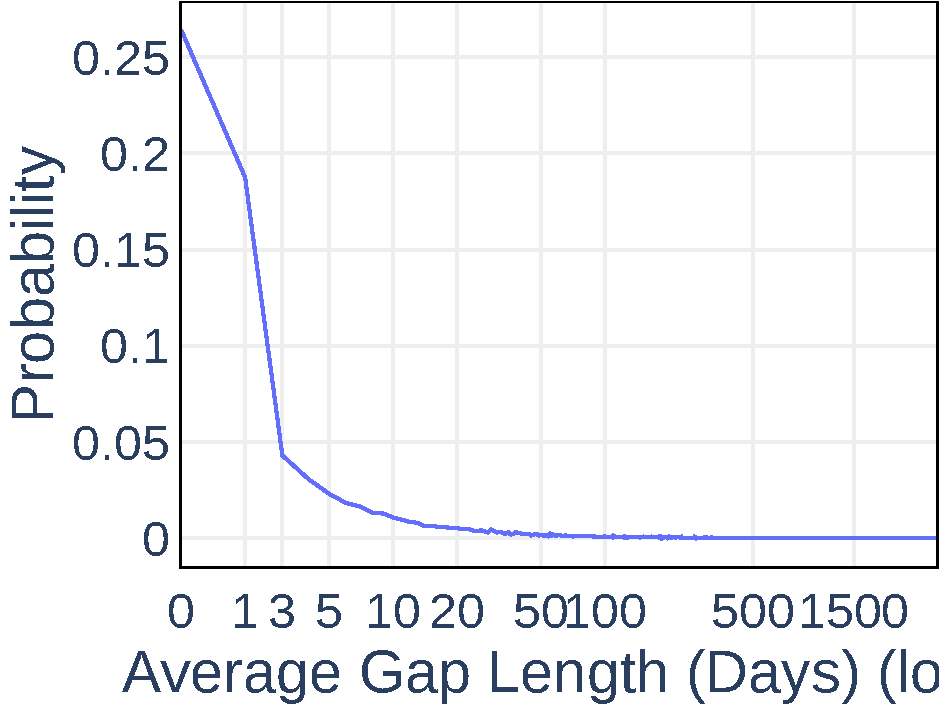
\includegraphics[width=\textwidth]{Figures/Data-AvgGapLen-PDF}
  \end{subfigure}
	% \begin{subfigure}[b]{0.3\textwidth}
    % 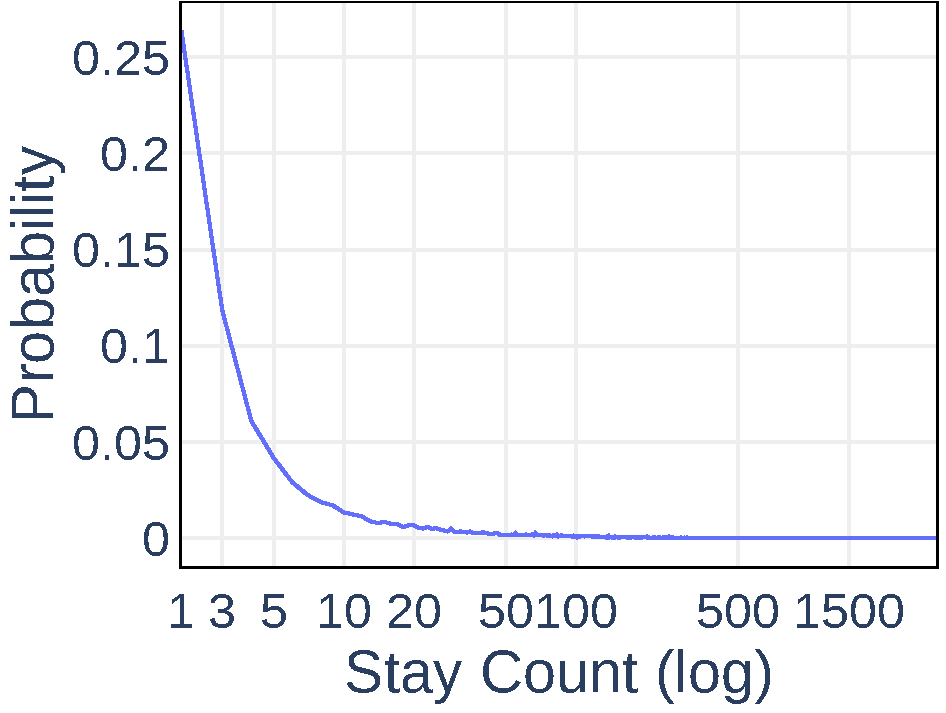
\includegraphics[width=\textwidth]{Figures/Data-TotalStays-PDF}
  % \end{subfigure}
	\begin{subfigure}[b]{0.3\textwidth}
    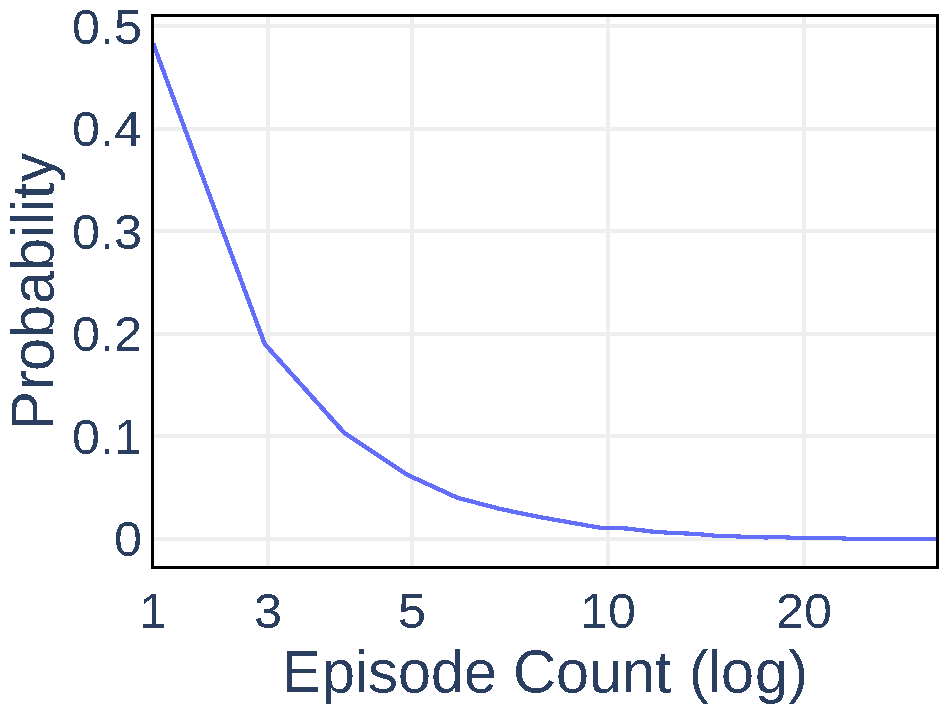
\includegraphics[width=\textwidth]{Figures/Data-TotalEpisodes-PDF}
  \end{subfigure}
	\caption{Histograms of the five Demographic fields.}
	\label{fig:demopdf}
\end{figure}


\section{Labelling the Data} \label{chap:data:labelling}

As stated in the introduction, the approach taken in this work is to identify clients that will eventually become chronic. There is no consensus for what it means to be chronically homeless, thus a definition must be selected. There are three "standards" that apply to our work, the Canadian federal definition, the Alberta provincial definition, and the definition applied by the DI. There are also several standards \cite{byrne2015testing} from other locations and organizations which will not be considered here. The three definitions under consideration are:

\begin{enumerate}
\item \textbf{Government of Canada (GoC):} "individuals who are currently experiencing homelessness AND who meet at least 1 of the following criteria: they have a total of at least 6 months (180 days) of homelessness over the past year or they have recurrent experiences of homelessness over the past 3 years, with a cumulative duration of at least 18 months (546 days)" \cite{canada2020definition}
\item \textbf{Government of Alberta (GoA):} "A person or family is considered chronically homeless if they have either been continuously homeless for a year or more, or have had at least four episodes of homelessness in the past three years." \cite{snyder2008albertadefinition}
\item \textbf{Calgary Drop-In Centre (DI):} "individuals who access the Calgary Drop-In Centre more than 75\% or 276 [sic] days in a calendar year" \cite{di_2019}.
\end{enumerate}

Of these three definitions, the DI definition was selected for use in this work. It was selected for two reasons. First, the DI definition most closely aligns with the original chronic classification \cite{kuhn1998applying}, as shown in our other work \cite{messier2020}. The second, and perhaps more functional reason, is that this work is being undertaken in partnership with the DI, and thus will use the internal definition of the DI.

Thus, for the remainder of this thesis, the term "chronic" will refer to chronic under the DI definition. In the context of homelessness, we interpret "access" as sleeps and do not include access to other DI services (which can be available to housed individuals). It is possible for a client to access the DI for both day and night sleeps, in this definition only a maximum of one sleep per 24 hour period is counted. Our analysis will be constrained to clients that spend at least one night (or day sleep) at the shelter. Of the 18,398 clients covered by this data set, only 886 (4.82\%) have ever met the DI definition for chronic homelessness.

The chronic label generated by applying the DI definition across the attribute table $A$ will be denoted $C$. Thus $C$ is a vector of boolean values corresponding to the chronic status of each client in $A$. To generate $C$ a rolling window of 365 days is applied to each client in $T$. The number of unique sleeps within any of those resulting windows is counted and if this number is greater than or equal to 276 nights, the client is identified as having experienced chronic homelessness. We note that this definition requires a recently homeless person to spend \emph{at least} 276 days sleeping in a shelter before being eligible for additional support based on chronic status.
While the minimum required time to be identified as chronic is 276 days, the median is 349 days and the mean is 666 days. These numbers are based on the data provided to us by the DI.
This effect was studied in our previous work \cite{messier2020} and motivates the need for a tool that considers a client's first $d$ days in shelter, where $d < 276$. $C$ will be used in later chapters as the class label for training procedures.

\subsection{Characteristics of Chronic Clients}

Following the discussion in Section \ref{chap:data:characteristics}, the same table structure will be presented here focusing only on clients that were identified as chronic using the DI definition (Table \ref{tbl:stats:chronic}). It can be seen that the median client who meets the definition of chronic has significantly more interactions than the general population (Table \ref{tbl:stats:notchronic}). Furthermore, as could be expected, the minimum number of sleeps is 276, and the minimum tenure is only slightly higher at 280. A new row, Tenure Pre-chronic, has been added to demonstrate the number of days a client is homeless before being identified as chronic. 

\begin{table}[h]
	\centering

	\begin{tabular}{lrrrr}
	\toprule
	Attributes &      min &      max &     mean &   median \\
	\midrule
	Age                          &       19 &       83 &    51.67 &       54 \\
	Bar (Count)                  &        0 &       68 &     5.21 &        2 \\
	CounsellorsNotes (Count)     &        0 &      443 &    26.34 &       17 \\
	EmployeeIsCounsellor (Count) &        0 &      464 &    58.78 &       32 \\
	EmsLogFlag (Count)           &        0 &       27 &     0.73 &        0 \\
	Log (Count)                  &        0 &     2419 &    62.23 &       21 \\
	PoliceLogFlag (Count)        &        0 &       11 &     0.34 &        0 \\
	ProgressDetails (Count)      &        0 &      539 &    45.37 &       30 \\
	Sleep (Count)                &      276 &     3575 &   955.06 &    787.5 \\
	\midrule
	Demographics								 &         &    &      &    \\
	\midrule
	Interactions (Count)         &      283 &     5247 &  1292.97 &   1091.0 \\
	Tenure (Days)                &      280 &     3800 &  1687.09 &     1636 \\
	Usage (\%)                    &  8.00225 &      100 &  63.6248 &  65.9663 \\
	Average Gap Length (Days)    &        1 &  12.5371 &  2.05862 &   1.5166 \\
	% Stays (Count)                &      276 &     3575 &  955.058 &    787.5 \\
	Episodes (Count)             &        1 &       22 &  3.69977 &        3 \\
	Tenure Pre-chronic (Days)    &      275 &     3623 &  665     &      349 \\
	\bottomrule
	\end{tabular}


	\caption{Basic Attribute statistics and Demographic data for chronic individuals.}
	\label{tbl:stats:chronic}
\end{table}


\section{Summary}

This chapter introduced the data set provided by the DI including the definitions used to label clients as chronic. Further, the attribute data and the demographic summaries were presented demonstrating some of the differences between chronic and non-chronic users of the DI. A discussion of classification evaluation measures will be presented in the following chapter.
